\section{Helmholzsche Wirbelsätze}

\subsection{Historisches}

Um das Verhalten von Wirbelringen besser zu verstehen, sind die sogenannten helmholzschen Wirbelsätze sehr nützlich. 
Mitte 19. Jahrhundert formulierte der Deutsche Physiker Hermann von Helmholtz 3 Wirbelsätze und veröffentlichte diese im Journal für die reine und angewandte Mathematik\cite{Wirbelringe:JournalHelmholz}.
In dieser definiert er auch gleich auch Hilfslinien, um die Wirbelbewegungen, besser beschreiben zu können:

\subsubsection*{Wirbellinien}

Wirbellinien sind die „Mittelachse“ eines Wirbels. 
Um diese Achse rotieren die Teile, welche teil eines Wirbels sind. 
Diese hat an sich kein Volumen, allerdings kann es sein das Teilchen auf dieser Achse zu liegen kommen. 

\subsubsection*{Wirbelfäden}



\subsection{Erster Helmholzscher Wirbelsatz}

\begin{displayquote}
    In Abwesenheit von wirbel anfachenden äusseren Kräften bleiben wirbelfreie Strömungsgebiete wirbelfrei.
\end{displayquote}

Teilchen die, ruhen bleiben in ruhe.

\begin{figure}
\centering
\includegraphics[width=0.4\textwidth]{papers/wirbelringe/fig/cube_still_particles.pdf}
\caption{Visuelle Darstellung des 1. helmholtzschen Wirbelsatz \label{buch:papers:Wirbelringe:fig:Helmholtz_1}}
\end{figure}

\subsection{Zweiter Helmholzscher Wirbelsatz}

\begin{displayquote}
    Fluidelemente, die auf einer Wirbellinie liegen, verbleiben auf dieser Wirbellinie.
\end{displayquote}

\begin{figure}
\centering
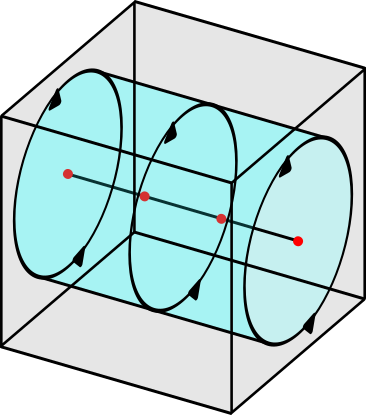
\includegraphics[width=0.4\textwidth]{papers/wirbelringe/fig/cube_still_particles_rotation.pdf}
\caption{Visuelle Darstellung des 2. helmholtzschen Wirbelsatz \label{buch:papers:Wirbelringe:fig:Helmholtz_2}}
\end{figure}

\subsection{Dritter Helmholzscher Wirbelsatz}

\begin{displayquote}
    Fluidelemente, die auf einer Wirbellinie liegen, verbleiben auf dieser Wirbellinie.
\end{displayquote}

\begin{figure}
\centering
\includegraphics[width=0.4\textwidth]{papers/wirbelringe/fig/cube_constant_rotation.pdf}
\caption{Visuelle Darstellung des 3. helmholtzschen Wirbelsatz \label{buch:papers:Wirbelringe:fig:Helmholtz_3}}
\end{figure}

\subsection{Verhalten an Grenzflächen}